\scanpage{61}
\diagram{\begin{tikzcd}[column sep=large]
\underbrace{\operatorname{Hom}(X_\bullet,P_\bullet)}\otimes_k
\underbrace{\operatorname{Hom}(Y_\bullet,Q_\bullet)}
\arrow[r]&\operatorname{Hom}(X_\bullet\boxtimes Y_\bullet,P_\bullet\boxtimes Q_\bullet)\\
Z^0(\check X_\bullet\otimes P)\otimes_k Z^0(\check Y_\bullet\otimes Q_\bullet)\arrow[r]&
\deleted{\unsure{Z^0(\check X_\bullet\operatorname{Hom}}}\,
Z^{00}\bigl((\check X_\bullet\boxtimes\check Y_\bullet)\otimes(P_\bullet\boxtimes Q)\bigr)
\end{tikzcd}}

\diagram{\begin{tikzcd}[column sep=small,row sep=small]
&&&0\arrow[d]\\
&&&k\arrow[d]\\
&&k\arrow[r,dash]\arrow[d]&k\\
&k\arrow[r,dash]\arrow[d]&k&\\
k\arrow[r,dash]&k&&\\
\cdots&&&
\end{tikzcd}}
\diagram{\begin{tikzcd}[row sep=small]
0\arrow[d]\\C^0\arrow[d]\\C^1\arrow[d]\\C^{\unsure{2}}\arrow[d]\\C^3\arrow[d]\\\vdots
\end{tikzcd}}
\[
Z_n(P_\bullet)\otimes Z_m(Q_\bullet)\simeq Z_{n,m}(P_\bullet\boxtimes Q_\bullet)
\]
\diagram{\begin{tikzcd}[column sep=small]
\deleted{\unsure{\Theta}}\ L'_{n+1}\arrow[r,dash]&L'_n\arrow[r,dash]&L'_{n-1}\\
\cdots\mathbin{\text{---}}L_{n+1}\arrow[r,"\sim"']\arrow[u]&L_n\arrow[u]\arrow[ul]\arrow[r,dash]&0
\end{tikzcd}}
\[
\operatorname{Hom}(k,L)\simeq L_0
\]
\[
\operatorname{Hom}(\Theta[n],L^{\unsure{\alpha}})\simeq L_{n+1}^{\unsure{F}}
\]
\[
\operatorname{Hom}(\Theta[m],L)\simeq L_{m+1}
\]
\deleted{$\operatorname{Hom}(\Theta[n],\unsure{\boxtimes}$}
\[
\operatorname{Hom}(\Theta[n]\boxtimes\Theta[m],P_\bullet\boxtimes Q_\bullet)
\simeq(P_{\unsure{n}}\boxtimes Q_m)_{\unsure{n+1,m+1}}
\]
\[
\operatorname{Hom}(\Theta[n]\boxtimes k,P_\bullet\boxtimes Q_\bullet)
\simeq(P_\bullet\deleted{\unsure{\otimes}}\boxtimes Q_\bullet)_{n,0}
\]
\[
\operatorname{Hom}\bigl(k\boxtimes\Theta[n],P_\bullet\boxtimes Q\bigr]
\simeq[P\boxtimes Q]_{0,n}
\]
\[
\operatorname{Hom}(k\boxtimes k,P_\bullet\boxtimes Q_\bullet)
\simeq[P_\bullet\boxtimes Q_\bullet]_{0,0}
\]
\figure{\begin{tikzpicture}\draw (0,0) .. controls (5,0.6) and (11,0.8) .. (15,0.25);\end{tikzpicture}}

\diagram{\begin{tikzcd}[column sep=small,row sep=small]
&0\\
k\arrow[r,dash,"\sim"]\arrow[ur,dash]&k\arrow[u]\arrow[r,dash]\arrow[d,"\unsure{2}"']&\phantom{k}\\
k\arrow[u,"\unsure{2}"]\arrow[uur,dash]\arrow[r,"\sim"]&k\arrow[ul,dash]&
\end{tikzcd}}
$\mathrm{Ch}_\bullet(\mathrm{Ab}_k)$

$\mathrm{Ch}$
\[
\mathrm{Ch}_\bullet(P^{\unsure{\flat|h}})\simeq
(\Lambda_\bullet\otimes_{\mathbf Z}P)^{\unsure{\flat|h}}
\]
\[
\mathbf P\qquad\mathrm{Ch}_\bullet\qquad\mathrm{Ch}_\bullet
\]
\figure{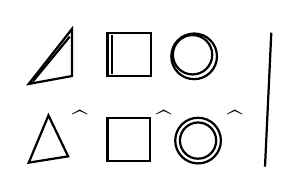
\begin{tikzpicture}[line width=0.8pt]
\draw (0,0)--(0.55,0.1)--(0.55,0.7)--cycle;
\draw (0.05,0.03)--(0.52,0.6);\draw (1,0.1)rectangle(1.55,0.65);
\draw (1.06,0.12)--(1.06,0.62);\draw (2.1,0.35)circle(0.29);
\draw (2.08,0.37)circle(0.25);
\draw (0,-1)--(0.5,-0.92)--(0.25,-0.4)--cycle;
\node at (0.65,-0.46) {$\widehat{\phantom{a}}$};
\draw (1,-0.98)rectangle(1.54,-0.43);\node at(1.72,-0.46){$\widehat{\phantom{a}}$};
\draw (2.15,-0.72)circle(0.29);\draw (2.15,-0.72)circle(0.23);
\node at(2.62,-0.46){$\widehat{\phantom{a}}$};\draw(3,-1.05)--(3.08,0.65);
\end{tikzpicture}}
$\mathrm{ch}_\bullet$
\[
\mathrm{ch}_\bullet^{\unsure{k}}\simeq\deleted{k\otimes}\mathrm{ch}_\bullet\otimes_{\mathbf Z}k
\]
\[
\mathrm{ch}_\bullet^{\unsure{\flat|h}}\simeq\mathrm{Ch}_\bullet(\mathrm{Ab})
\]
\[
\mathrm{ch}_{\bullet A}^{\deleted{\unsure{\flat}}\unsure{\sharp}}\simeq\mathrm{Ch}_\bullet(A)
\]
\[
\mathrm{ch}_\bullet\otimes\mathrm{ch}_\bullet\simeq
\text{\inserted{bi}complexe de chaînes}
\]
\[
\mathrm{ch}_{\bullet A^{\unsure{\flat}}}^{\unsure{\flat}}
\simeq\mathrm{Ch}_\bullet(A^{\unsure{\flat}})\simeq
\deleted{\unsure{A}}(\mathrm{ch}_\bullet\otimes_{\mathbf Z}A)^{\unsure{\sharp}}
\]
\margin{\figure{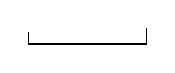
\begin{tikzpicture}\draw(0,0.15)--(0,0)--(1.5,0)--(1.5,0.2);\end{tikzpicture}}
complexes de chaînes dans $A$ qui sont homotopes à un complexe constant}
\[
\overset{n}{\bigotimes}\mathrm{ch}_\bullet=\mathrm{ch}_{(n)}
=\mathrm{ch}\deleted{\unsure{_{n,n}}}
\]
$\mathrm{Ch}_\bullet$
\[
\deleted{\unsure{\mathrm{ch}_\bullet^A\simeq}}\ \simeq\mathrm{ch}_\bullet\otimes_{\mathbf Z}A
\]
\mspage{60}
